%%%%%%%%%%%%%%%%%%%%%%%%%%%%%%%%%%%%%%%%%%%%%%%%%%%%%%%%%%%%%%%%%%%%%%
% Lớp 10 | Bất phương trình bậc 2 một ẩn | Dấu của tam thức bậc 2
% Dạng 0D7?1-4: Xét dấu biểu thức dạng tích, thương
% Số câu: 6  (sinh tự động bởi tach_cau.py; từ nay thầy sửa trực tiếp file này)
%%%%%%%%%%%%%%%%%%%%%%%%%%%%%%%%%%%%%%%%%%%%%%%%%%%%%%%%%%%%%%%%%%%%%%

%%%%%%%%%%%%%%%% TRẮC NGHIỆM 4 PHƯƠNG ÁN %%%%%%%%%%%%%%%%

% nguồn: MaHoaNH_TracNghiem_Lop10
\begin{ex}%[0D7H1-4]%[ma:eb915c30]
	Tập nghiệm bất phương trình $\left(9-x^{2}\right)(2x-10)<0$  là
	\choice 
		{$(-\infty;-3)\cup(3;5)$} 
		{$(-\infty;-3)\cup(5;+\infty)$} 
		 {$(-3;3)$}
		{\True  $(-3;3)\cup(5;+\infty)$}
	\loigiai{ 
		 Xét $\left(9-x^{2}\right)(2x-10)=0\Leftrightarrow\hoac{&x=\pm 3\\&x=5.}$\\
		 Bản xét dấu
		\begin{center}
			\begin{tikzpicture}
					\tkzTabInit[nocadre=true,lgt=3,espcl=2,deltacl=0.5] 
						{$x$/0.7,$9-x^2$/0.7,$2x-10$/.7,$(9-x^2) 
						 (2x-10)$/.7}
						{$-\infty$,$-3$,$3$,$5$,$+\infty$} 
					\tkzTabLine{,-,$0$,+,$0$,-,|,-,} 
					 \tkzTabLine{,-,|,-,|,-,$0$,+,}
					 \tkzTabLine{,+,$0$,-,$0$,+,$0$,-,}
				\end{tikzpicture}
		\end{center}
		Dựa  vào bảng xét dấu, suy ra $\left(9-x^{2}\right)(2x-10)<0$ khi $x\in(-3;3)\cup(5;+\infty)$.\\
		Vậy tập nhiệm của  bất phương trình $\left(9-x^{2}\right)(2x-10)<0$ là $(-3;3)\cup(5;+\infty)$.
	 }
\end{ex}

% nguồn: MaHoaNH_TracNghiem_Lop10
\begin{ex}%[0D7H1-4]%[ma:da13e1f7]
	Gọi $ S $ là tập nghiệm của bất phương trình  $\dfrac{x^2 - 2x + 1}{x^2 - 9} \geq 0.$
	Khi đó $S\cap (-3;3) $  là tập nào sau đây?
	\choice 
		{$(-3;1]$} 
		 {$(-3;3)$}
		{$(-3;0)$} 
		{\True $\{1\}$} 
	 \loigiai{
		Ta có tử số $x^2 - 2x +  1= (x-1)^2 $ luôn không âm và bằng 0 khi $ x = 1 $.\\
		 Từ bất phương trình $f(x)=\dfrac{(x-1)^2}{(x-3)(x+3)} \geq 0$. Ta có bảng xét dấu
		\begin{center}
			\begin{tikzpicture}
					\tikzset{t  style/.style={style=draw}}
					 \tkzTabInit[deltacl=0.5,espcl=2.5,lgt=2,nocadre]
						 {$x$/1,$(x-1)^2$/1,$(x-3)$/1,$(x+3)$/1,$f (x)$/1}
						{$8$,$-3$,$1$,$3$,$8$} 
					 \tkzTabLine{,+,,+,0,+,,+,}
					\tkzTabLine{,-,,-,,-,0,+,} 
					\tkzTabLine{,-,0,+,,+,,+,} 
					 \tkzTabLine{,+,||,-,0,-,||,+,}
				\end{tikzpicture}
		\end{center}
		$\Rightarrow S=\left(-\infty;  -3\right)\cup \left(3;+\infty\right)\cup \{1\}$.\\
		Vậy $ S \cap (-3;3) = \{1\}  $.
	} 
\end{ex}

% nguồn: MaHoaNH_TracNghiem_Lop10
\begin{ex}%[0D7H1-4]%[ma:6947e064]
	Tìm  tập nghiệm của bất phương trình $\dfrac{x^{2}-3x-4}{x-1}\leq 0$.
	\choice 
		 {$T=(-\infty;-1]\cup[1;4]$}
		 {\True $T=(-\infty;-1]\cup(1;4]$}
		 {$T=(-\infty;-1)\cup(1;4]$}
		{$T=(-\infty;-1]\cup(1;4)$} 
	 \loigiai{
		Xét biểu  thức $f(x)=\dfrac{x^{2}-3x-4}{x-1}$.\\
		 Ta có
		\begin{itemize}
			 \item $x^{2}-3 x-4=0\Leftrightarrow\hoac{&x=-1\\&x=4.}$
			\item $x-1=0 \Leftrightarrow  x=1$.
		\end{itemize}
		Bảng xét dấu 
		\begin{center}
			\begin{tikzpicture}
					 \tkzTabInit[nocadre=true,lgt=2.5,espcl=2,deltacl=0.5]
						{$x$/0.7,$x^2-3x-4$/0.7,$x-1$/.7,$f  (x)$/.7}
						{$-\infty$,$-1$,$1$,$4$,$+\infty$} 
					 \tkzTabLine{,+,$0$,-,|,-,$0$,+,}
					\tkzTabLine{,-,|,-,0,+,|,+,} 
					\tkzTabLine{,-,$0$,+,||,-,$0$,+,} 
				\end{tikzpicture}
		\end{center}
		Từ bảng xét dấu, suy ra  $f(x)\leq0\Leftrightarrow x\in (-\infty;-1]\cup(1;4]$.\\
		Vậy tập nghiệm của bất phương  trình đã cho là $T=(-\infty;-1]\cup(1;4]$.
	} 
\end{ex}

% nguồn: MaHoaNH_TracNghiem_Lop10
\begin{ex}%[0D7H1-4]%[ma:17226eed]
	Cho biểu thức $f(x)=x^2 \left(x^2-4\right)$ có bảng xét dấu như  sau
	\begin{center}
		\begin{tikzpicture}[>=stealth]
				\tkzTabInit[nocadre=false,lgt=1.5,espcl=2,deltacl=0.6]{$x$/.7,$f (x)$/.7} 
					 {$-\infty$,$-2$,$0$,$2$,$+\infty$}
				\tkzTabLine{,?,$0$,?,$0$,?,$0$,?,} 
			\end{tikzpicture}
	\end{center}
	 Dấu trong các dấu chấm hỏi theo thứ tự từ trái sang phải là
	\choice 
		{\True  $+,-,-,+$}
		 {$+,-,+,-$}
		{$-,+,-,+$} 
		 {$+,+,-,+$}
	\loigiai{ 
		Ta có $f(x)=0\Leftrightarrow \hoac{&{x=0}  \\
		&{x=\pm  2.}
		 &}$\\
		Ta có bảng xét dấu $f(x)=x^2\left(x^2-4\right)$  như sau
		\begin{center}
			\begin{tikzpicture}[>=stealth]
					 \tkzTabInit[nocadre=false,lgt=1.5,espcl=2,deltacl=0.6]{$x$/.7,$f (x)$/.7}
						 {$-\infty$,$-2$,$0$,$2$,$+\infty$}
					\tkzTabLine{,+,$0$,-,$0$,-,$0$,+,} 
				\end{tikzpicture}
		\end{center}
		 Do đó các dấu chấm hỏi theo thứ tự từ trái sang phải là $+,-,-,+$.
	 }
\end{ex}

% nguồn: MaHoaNH_TracNghiem_Lop10
\begin{ex}%[0D7V1-4]%[ma:3b7ce660]
	Cho  biểu thức $f(x)=\dfrac{\left(x^2-4x+4\right)\left(x+3\right)}{5x}$. Trong khoảng $\left(0;2\right)$, $f(x)$ mang dấu gì?
	\choice 
		{\True dương} 
		 {âm}
		{không dương} 
		 {không âm}
	\loigiai{ 
		Ta có 
		\begin{itemize}
			 \item $x^2-4x+4=0\Leftrightarrow x=2$.
			 \item $x+3=0\Leftrightarrow x=-3$.
			\item $5x=0\Leftrightarrow  x=0$.
		\end{itemize}
		Bảng xét dấu 
		\begin{center}
			\begin{tikzpicture}[>=stealth]
					\tkzTabInit[nocadre=false,lgt=3]{$x$/.7,$x^2-4x+4$/.7,$x+3$/.7,$5x$/.7,$f (x)$/.7} 
						 {$-\infty$,$-3$,$0$,$2$,$+\infty$}
					\tkzTabLine{,+,t,+,t,+,$0$,+,} 
					 \tkzTabLine{,-,$0$,+,t,+,t,+,}
					\tkzTabLine{,-,t,-,$0$,+,t,+,} 
					\tkzTabLine{,+,$0$,-,$0$,+,$0$,+,} 
				\end{tikzpicture}
		\end{center}
		Từ  bảng xét dấu, ta thấy trong khoảng $\left(0;2\right)$, $f(x)$ mang dấu dương.
	 }
\end{ex}


%%%%%%%%%%%%%%%% ĐÚNG/SAI %%%%%%%%%%%%%%%%

% nguồn: MaHoaNH_DungSai_Lop10
\begin{ex}%[0D7V1-4]%[ma:7ac19e37]
	Cho $f(x)=\dfrac{5 x^2+3 x-8}{x^2-7 x+6}$. Khi  đó
	 \choiceTF
		{Điều  kiện $x\neq 6$}
		{$f(x)=0 \Rightarrow x=1$  hoặc $x=-\dfrac{8}{5}$}
		{\True $f(x)>0, \forall x  \in\left(-\infty;-\dfrac{8}{5}\right) \cup(6;+\infty)$}
		{\True $f(x)<0, \forall x  \in\left(-\dfrac{8}{5}; 1\right) \cup(1; 6)$}
	 \loigiai{
		\begin{itemchoice}
			 \itemch
			Điều kiện $x^2-7x+6 \ne 0 \Leftrightarrow  \heva{&x\ne 1\\& x \ne 6.}$
			 \itemch
			Xét $f(x)=0  \Rightarrow 5x^2+3x-8=0 \Rightarrow \hoac{&x=1 \text{ (loại)}\\&x=-\dfrac{8}{5} \text{ (nhận)}}$.\\
			Vậy $x=-\dfrac{8}{5}$. 
			\itemch Ta  có\\
			Bảng xét  dấu
			\begin{center}
				\begin{tikzpicture}[>=stealth]
						 \tkzTabInit[lgt=4,espcl=3]
						 {$x$ /1,$5x^2+3x-8$ /1,$x^2-7x+6$ /1,$f (x)$ /1}
						 {$-\infty$,$-\dfrac{8}{5}$,$1$,$6$,$+\infty$}
						\tkzTabLine{,+,0,-,0,+,t,+,} 
						 \tkzTabLine{,+,t,+,0,-,0,+,}
						\tkzTabLine{,+,0,-,d,-,d,+,} 
					\end{tikzpicture}
			\end{center}
			Kết luận: $f(x)>0,  \forall x \in\left(-\infty;-\dfrac{8}{5}\right) \cup(6;+\infty)$.
			\itemch 
			 $f(x)<0, \forall x \in\left(-\dfrac{8}{5}; 1\right) \cup(1; 6)$.
	\end{itemchoice}}
\end{ex}
